% Chapter 2

\chapter{Background} % Chapter title

\label{ch:background} % For referencing the chapter elsewhere, use \autoref{ch:background} 

%----------------------------------------------------------------------------------------

In this chapter, we are going to review the history of the \emph{Multi-level Security} (MLS), its definitions, usages, and one of its most famous models: the Bell-LaPadula model.
MLS is a very famous solution for the security problems of multiple subjects accessing one shared system. 
Studying it will open various paths to the information security solutions.
We can see how we can keep the system forcefully secured; 
how we can divide the system into different levels, each of which has corresponding policies, to archive the security requirements comprehensively.
\marginpar{In MLS systems, there are only \emph{subjects} and \emph{objects}, which have various \emph{properties} called \emph{clearance} and \emph{classification}} 
Moreover, MLS defines objective relations between multi-level users with the system assets. 
Additionally, we also see how those advantages are designed in BLP model, as well as its ideas of an MLS system.

%----------------------------------------------------------------------------------------

\section{Multi-level Security}
\label{ch:background:mls}

Since the very early time of computer era, from 1960s, the need of communicating and sharing information among users within a same system was already tremendous.
Along with the raise of the number of services and connected devices, information security is becoming paramount in organizations, especially governments, intelligent agents, etc...
The event of secret data is brought public may lead to various levels of damage.
In consideration of issues caused by the failure, \citeauthor{centos:2008} \cite{centos:2008} cited that:

\begin{quote}
Businesses may face legal or financial ramifications. At the very least, they will suffer a loss of customer trust. 
In most cases, however, they can recover from these financial and other losses with appropriate investment or compensation. 
The same cannot be said of the defense and related communities, which includes military services, intelligence organizations and some areas of police service.
These organizations cannot easily recover should sensitive information be leaked, and may not recover at all. 
\end{quote}

In every organization, there is very likely a central system everyone with different roles can login and access data in it.
While some pieces of data are not so vital, they can be viewed or edited by anyone in the team, the others could be only essential to be available to a small group of particular people who are more influential, or in charge of making decisions.
So that, as the managerial platitudes, the \emph{security policy} is critical to achieve that control.

\citeauthor{ross:2008}, in \cite{ross:2008}, defined the security policy as
\begin{quote}
a document that expresses clearly and concisely what the protection mechanisms are to achieve. It is driven by our understanding of threats, and in turn drives our system design.
\end{quote} 
The security policy does not only specify the system protection requirements, but it may also be a part of the system specification.
Technically, the security policy should emphasize the ``need-to-know'' statements.
It should represent the conditions for a user (or a group of users with common characteristics) to get permission on the properties they request in the system.

\emph{Multi-level security} (MLS) is a security model which ensures principals with multiple clearance level can read and write to the system assets whose clearance level satisfies the predefined security policies. 

According to \citeauthor{bancinco:2015} \cite{bancinco:2015}, under MLS, users and machine processes are called \emph{subjects}, and files, devices and other passive components of the system are called \emph{objects}.
So, MLS is a system design which allows multiple subjects (users) with difference clearance levels can access objects (data) flowing in the system while restricting their accesses corresponding to their clearance (or security level) \eg\ Unclassified, Confidential, Secret, Top Secret\dots
For example, in BLP model, in regard to reading permission, Secret subjects can only access to Secret or lower security level objects.

\begin{figure}[bth]
\myfloatalign
\includegraphics[width=1.0\linewidth]{gfx/chapter_2/security_level_read_example}
\caption[BLP: Security Levels read examples]{BLP: Security Levels read examples}\label{fig:security_level_read_example}
\end{figure}

Rather than that, a successful MLS system should allow various subjects to access and share objects to other chosen subjects.
The object owners should not be in charge of making decision whom they grant access to their assets. 
\citeauthor{prasun:1996} \cite{prasun:1996} called this kind of control \emph{discretionary access control} (DAC).
DAC is hard for the owner to manage access right when the number of his objects becomes huge, also some of them are too old to remember, and this consequently causes data leaks or mis-use.
Hence, MLS design should \emph{force} subjects and all of their objects to follow the set of \emph{predefined rules}.
This is called the \emph{mandatory access control} (MAC), and it automates a great port of the access control throughout the system.

Moreover, security levels sometimes are not enough to prevent someone gaining permission to pieces of data.
Let us consider this example. 
In one organization, at the same security level, there will be many people with different roles who may need different data.
Allowing everyone with the same security level access to data of the other roles is considered redundant.
It causes confusion to other users about which data is related to them and what they can actually use.
Furthermore, in some point of view, it poses security threads to leak out secret data of a department to the others and vice versa.
As the result, MLS need to segregate users and the organization assets into specific groups of roles \eg\ Project Manager, Designer, Programmer etc...
It is called \emph{classification}.
Unlike clearance, every subjects can have more than one classification.
It reflects the real scenarios in organizations where one person may have more than one roles.
By classifying users, MLS can ensure that users can only receive what is necessary for them to finish their jobs, no more no less.

\emph{Clearance} and \emph{classification} assigned to a subject, then, are called \emph{labels}.
By combining these two kinds of label and the \emph{access permissions} (read and write), the system can easily control the data flow in the system.
It can actively decide which pieces of data conform to a particular subjects or a group of relating ones and how they can interact with it (read or write).
The users can, then, gain the access permission to data which full-fills predefined rules.
For instance, with BLP model which we are going to study more in \autoref{ch:background:bell}, an object is labeled as \emph{Secret} for clearance, and \emph{Programmer} and \emph{Designer} with \emph{read} permission can only be \emph{viewed} by subjects who have \emph{Secret} or higher clearance, and one of two label \emph{Programmer}, \emph{Designer} or both, and they cannot modify it.

\begin{figure}[bth]                                                                                                                                                  
\myfloatalign
\includegraphics[width=1.0\linewidth]{gfx/chapter_2/mls_example}
\caption[BLP: MLS examples]{BLP: MLS examples}\label{fig:mls_example}
\end{figure}

In conclusion, MLS can be applied to business to ensure the data integrity of the company.
\emph{Category} and \emph{Security Level} together form various combinations which help to secure our data access, and to be able to predict the system data flow.
\graffito{Information Security is an adjustment between security and convenience, there is no \emph{single answer to all questions}.}
There are many MLS models, each of them is a different set of predefined rules, which has different pros and cons.
People should research about security models to select or adjust a suitable one for their system. 
In the next sections, I will go in more detailed about some MLS models, and put them in comparison in order to explain my decision of selecting the one is used in my project management platform.

%----------------------------------------------------------------------------------------

\section{Data Confidentiality (Bell-LaPadula model)}
\label{ch:background:bell}

\emph{Bell-LaPadula} (BLP) is a MLS model which was developed by Bell and LaPadula.
\citeauthor{ross:2008} \cite{ross:2008} stated that it \begin{quote}was proposed in 1973, in response to US Air Force concerns over the security of time-sharing mainframe system\end{quote}
BLP only takes the data confidentiality into account.
It decides \emph{who ``need-to-know''}, and prevents data leak to insufficient person.

As I mentioned in \autoref{ch:background:mls}, MLS combines usages of two kinds of label: \emph{clearance} (or \emph{security level}) and \emph{classification} (or \emph{role}).
Hence, BLP model endorse those components, and defines a set of rules for them to collaborate in the system.
According to \cite{ross:2008}, BLP enforces two properties:
\begin{description}
\item[Simple security property] no process may read data at a higher level, as known as \emph{no read up}
\item[*-property] no process may write data to a lower level, as known as \emph{no write down}
\end{description}
It means that users with higher security label can read data with lower security label, but not vice versa.
And so on, a user with lower security label can write to data with higher security label, however the higher security label can not.
The *-property was the critical innovation of BLP model.
It ensures that no data can flow down.
In the context of the project management platform, a secret level employee may unintentionally leave customer financial information where lower security level ones can access to it.
\emph{No-write-down} property, then, enforces all data written by secret level employee will be label at least as secret.
Consequently, uncleared can not access it throughout the system.

Let us call $S1$ security level of a subject, and $S2$ security level of an object, where 
$$S1,S2 \in \{top secret, secret, confidential, unclassified\}$$ 
and 
$$top secret > secret > confidential > unclassified$$
So the subject can read the object only if $S1 \geq S2$.
And it can write to the object only if $S1 \leq S2$.

As the result, the important data (data with high security label) can only be viewed by users with higher or the same importance.
And high security level user cannot leak important data to insufficient users, because they \emph{cannot write down}. 
\autoref{fig:blp_security_level_rules} shows the principles of handling request from a subject to the other objects regarding only to their security levels.

\begin{figure}[bth]
\myfloatalign
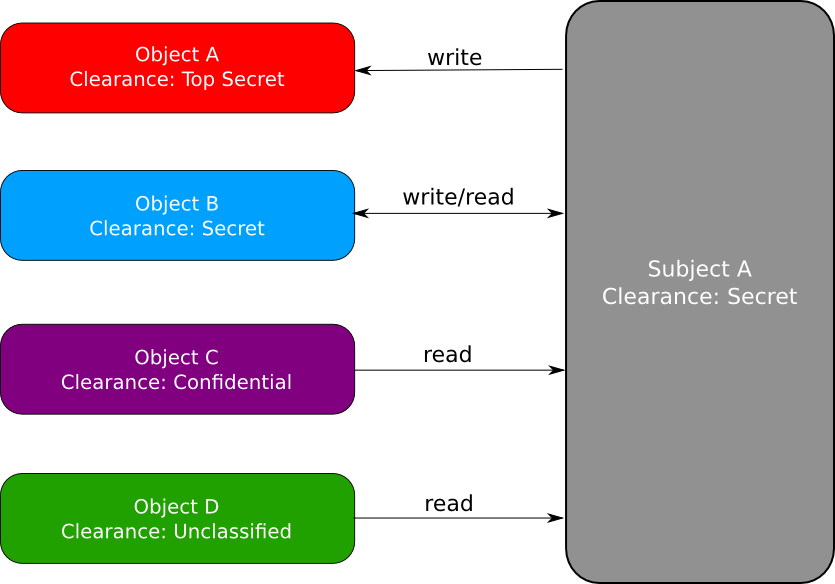
\includegraphics[width=1.0\linewidth]{gfx/chapter_2/blp_security_level_rules}
\caption[BLP: Security Level rules]{BLP: Security Level read/write rules}
\label{fig:blp_security_level_rules}
\end{figure}

In addition to security level labels, as mentioned above, BLP can also be designed in combination with \emph{classification} labels to create a stronger restriction to object accesses.
It is ``need-to-know'' principle.
Under the circumstances, the subject classification labels should be a subset of the object classification labels to be able to gain the access permission.
If we call the subject roles a set $R1$ and the object roles $R2$, where

$$R1, R2 \in \{project manager, programmer, designer\}$$ 

The subject can gain access permission to R2 only if $R1 \subseteq R2$.
\autoref{fig:blp_security_level_roles_rules} shows the principles of handling request from a subject to the other objects regarding only to their security levels.

\begin{figure}[bth]
\myfloatalign
\includegraphics[width=1.0\linewidth]{gfx/chapter_2/blp_security_level_roles_rules}
\caption[BLP: A set of Security Level and Roles rules]{BLP: A set of Security Level and Roles rules}
\label{fig:blp_security_level_roles_rules}
\end{figure}

Finally, a user can use \emph{Discretionary Access Control} (DAC) set the permission to an object.
\cite{centos:2008} cited that MLS access rules are always combined with \emph{conventional access permissions} (or file permission).
It means that if a user with security label \emph{Secret} uses DAC to block access to an object by the other uses, this also block access by by users with security level of \emph{Top Secret}.
Additionally, \cite{bancinco:2015} presented that
\begin{quote}
SELinux MLS policy rules are checked after DAC rules. A higher security clearance does not automatically give permission to arbitrarily browse a file system.
\end{quote}
Hence, \autoref{fig:blp_full} will be a mostly complete picture describing about BLP model after we put every components together.

\begin{figure}[bth]
\myfloatalign
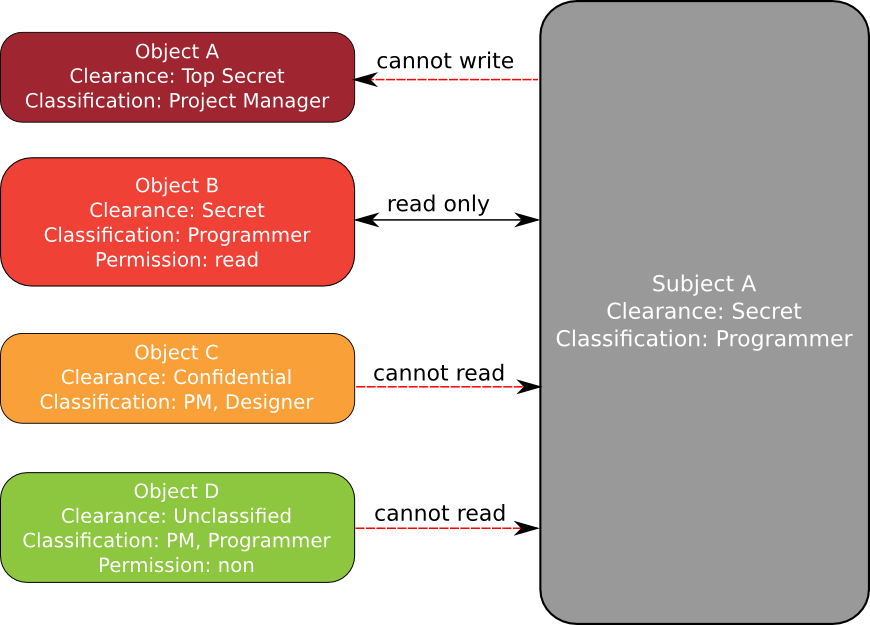
\includegraphics[width=1.0\linewidth]{gfx/chapter_2/blp_example}
\caption[BLP: all components illustration]{BLP: all components illustration}
\label{fig:blp_full}
\end{figure}

Although its benefits in system secure, BLP has some disadvantages in usage.
First of all, *-property only allows data to flow up.
In my own opinion, it is not so handy for management.
Because, subjects at higher level label can not send down commands to subjects of lower level label.
For instance, a project manager whose security label \emph{Secret} can not create tickets for lower level label team members.
As reported in \cite{ross:2008}, John McLean, in order to get over the difficulty, introduced \emph{System Z}.
System Z was defined as a BLP system with an additional feature that a user can ask the system administrator to temporarily reduce any objects to a lower security level label \ie from high to low.
In my own opinion, the \emph{System Z} violated the BLP properties.
It also gives the administrators too much power on the system data.
I personally think that it is a fraud of the system.
The system administrator should be viewed as the other subjects in the system, which means that they are also labeled with a specific security level.
Besides that, they should only work with the subjects labeling, not the objects.
In other words, administrator can change subject labels; 
then subjects in the system will be in charge of modifying the system objects, which is strictly enforced by the security policies.
Other limitations of the BLP models in management environment will be discussed later in \autoref{ch:background:security_model_in_hotpot} and \autoref{ch:hopot_project:concepts:security_features} where I explain my project implementation.

%----------------------------------------------------------------------------------------

\section{Data Integrity (Biba model)}
\label{ch:background:biba}

\emph{Biba} model is contrast to the Bell-LaPadula model.
Although it has a similar structure to BLP, Biba focuses toward data integrity rather than confidentiality.
According to \citeauthor{michael:2012}, in \cite{michael:2012}, the Biba model was originally published in 1977.
Biba model has similar structure to the BLP model in which they both use subjects, objects and labeling to control the data flow;
\cite{micki:1997} stated that 
\begin{quote}
It (Biba model) controls object modification in the same way that Bell-LaPadula controls disclosure
\end{quote}
Biba has three properties:
\begin{description}
\item[Simple integrity property] a subject at one integrity level can not read an object of lower level, as known as \emph{no read down}
\item[* integrity property] a subject at one integrity level can not write to an object of higher level, as known as \emph{no write up}
\item[Invocation property] a subject at one integrity level can not invoke another subject at a higher integrity level.
\end{description}
The first two are similar to BLP, however in the reversed way.
\emph{*-integrity-property} enforces that a subject at an \emph{integrity level} is can only modify objects at lower integrity level.
It ensures the subject only makes authorized changes, hence protects the object integrity.
For example, a project owner can write a features list for a team leader.
In this fashion, the team leader issues these features as tasks to his team members.
Conversely, the team member can not create task for his team leader or project owner.
As the result, the integrity of the project is assured.

Let us call $S1$ integrity level of a subject, and $S2$ integrity level of an object, where 
$$S1,S2 \in \{top secret, secret, confidential, unclassified\}$$ 
and 
$$top secret > secret > confidential > unclassified$$
So the subject can write to the object only if $S1 \geq S2$.
And it can read the object only if $S1 \leq S2$.

%----------------------------------------------------------------------------------------

\section{Security Model in HotPot}
\label{ch:background:security_model_in_hotpot}

\myProject is a \emph{project management platform} (PMP).
The system should protect both data confidentiality and integrity.
However, mixing two models may be complex and costly.
In my own opinion, in the context of management, data confidentiality should have slightly higher priority than data integrity.
In the system, there is data from various source \eg customer financial data, private server information\dots
These types of data should be protected, since leaking them will cause critical damages \eg money loss, system attack, user data leak, or losing the company reputation\dots 
Moreover, project management (PM) is an environment that need to be flexible to change. 
For instance, in the first stage of a project, the features list is very likely updated.
The team members, on the developing progress, will consult the customer to add or remove features.
In addition, when a critical issue hits, any team members should be able to create tickets to a higher security level member to diagnose it.
So that, maintaining data integrity in project management sometimes may decrease the flexibility of the management.
In order to ensure above criteria, I decided to use BLP model to develop my project.
However, there are functions in the system, which are not covered by the theory of the BLP model such as delete action, and visually editing a document.

In my experience, delete action is considered as data modification.
So that, it should follow \emph{*-property} logic.
However, thinking about the data integrity, the data owner should be the only one to be able to delete his data.
If any authorized users can delete cleared data, it could lose data unintentionally.
For instance, a technical note of a team leader can be deleted by a team member who thinks it's redundant.

Moreover, edit action should definitely follow *-property.
However, in my point of view, most of edit actions taken inside PMP are performed visually.
It means that the user should be able to view the document contents while editing it, rather than overwrite it blindly.
This is a challenge to implement MLS into PMP.
My solution for it is to enforce modification actions to follow both BLP properties.
What I mean is any subjects need to have the similar security label to an object to modify it.
Detailed explanation about this solution will be discussed later in \autoref{ch:hopot_project:concepts:security_features}.

In conclusion, MLS and BLP model, in specification, are suitable for the business systems, especially in my project \myProject.
It can isolate objects by labeling and protect them in multi-level accesses.
Furthermore, it provides a transparent working environment where users only get data that they ``need-to-know''.
